\documentclass[pdflatex,sn-mathphys-num]{sn-jnl} 

\usepackage{graphicx}
\usepackage{multirow}
\usepackage{amsmath,amssymb,amsfonts}
\usepackage{amsthm}
\usepackage{mathrsfs}
\usepackage[title]{appendix}
\usepackage{xcolor}
\usepackage{textcomp}
\usepackage{manyfoot}
\usepackage{booktabs}
\usepackage{algorithm}
\usepackage{algorithmicx}
\usepackage{algpseudocode}
\usepackage{listings}


\theoremstyle{thmstyleone}
\newtheorem{theorem}{Theorem}
\newtheorem{proposition}[theorem]{Proposition}

\theoremstyle{thmstyletwo}
\newtheorem{example}{Example}
\newtheorem{remark}{Remark}

\theoremstyle{thmstylethree}
\newtheorem{definition}{Definition}

\raggedbottom


\begin{document}

\title[Article Title]{Low-Code}




\abstract{Este artigo científico investiga o crescente fenómeno do desenvolvimento de software através da abordagem \textit{Low-Code}. Discutimos a relevância crescente do \textit{Low-Code} no cenário tecnológico atual, enfatizando o seu papel na simplificação do processo de desenvolvimento e na redução da lacuna entre os desenvolvedores e os utilizadores finais. Além disso, exploramos as implicações sociais do \textit{Low-Code}, destacando o seu potencial para promover a inclusão digital e capacitar comunidades menos privilegiadas ao fornecer ferramentas acessíveis para criar aplicações personalizadas. Analisamos as tecnologias comercialmente disponíveis no campo do \textit{Low-Code}, destacando a sua variedade e flexibilidade para atender às diversas necessidades de desenvolvimento. Também examinamos como a inteligência artificial está a ser implementada para com plataformas \textit{Low-Code}, melhorando a automação e a eficiência no processo de desenvolvimento. Por fim, abordamos a interface intuitiva de \textit{Drag\&Drop}, uma característica fundamental do \textit{Low-Code} que simplifica a criação de aplicações, permitindo que até mesmo utilizadores sem experiência técnica possam desenvolver soluções funcionais. Este estudo destaca o potencial transformador do \textit{Low-Code} na democratização do desenvolvimento de software, apontando para uma era de inovação mais acessível e inclusiva.}




\keywords{Low-Code, No-Code, Drag\&Drop, Desenvolvimento Eficiente, Inteligência Artificial, ChatBot, OutSystems, Zoho Creator}



\maketitle

\section{Introdução}\label{sec1}
O \textit{Low-Code}, pelo o que o próprio nome indica, é uma ferramenta de desenvolvimento de \textit{software} que permite a criação de aplicações com pouco ou nenhum código, como tal implica que o desenvolvimento das aplicações seja mais rápida, o que pode causar uma redução da equipa de desenvolvedores, que subsequentemente reduz o custo de desenvolvimento. O \textit{Low-code} permite ainda, que não seja necessário um curso superior para trabalhar com esta ferramenta, uma vez que não é preciso saber programar para usar ferramentas relacionadas ao \textit{Low-Code}.


\section{O que é Low-Code}\label{sec2}

\begin{center}
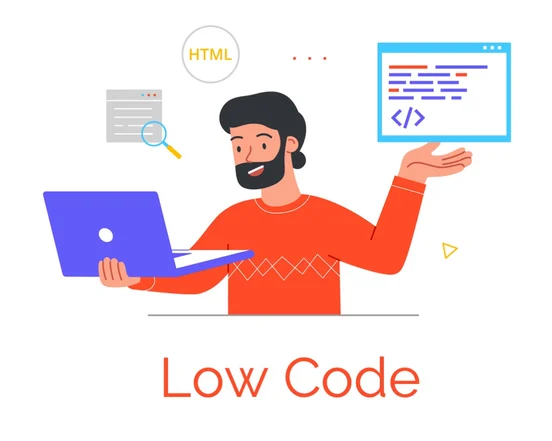
\includegraphics[width=0.75\textwidth]{Low Code Citizen Developer.jpg}
\end{center}


O \textit{low-code} é uma abordagem revolucionária no desenvolvimento de software projetada para simplificar e acelarar o processo de criação de aplicações, consistindo na utilização de elementos pré-definidos que podem ser arrastados para a tela (\textit{Drag\&Drop}) e interligados entre si, efetivamente permitindo que esses elementos cooperem de forma lógica para que se chegue ao pretendido. Isto permite que desenvolvedores e até mesmo utilizadores sem experiência em programação projetem e construam soluções, neste mesmo contexto também existe o conceito de \textit{nocode}, que é uma versão mais extrema do conceito de \textit{low-code}.\cite{bib4}

\paragraph{} Para tal há a necessidade de obtenção de formação na própria plataforma, mas tal formação é factualmente muito mais rápida e intuitiva do que a formação necessária para o domínio de qualquer linguagem de programação convencional -  Domínio esse visado ao mesmo nível que seria comparativamente necessário para o desenvolvimento da mesma qualidade e efetividade das soluções de software desenvolvidas. \cite{bib4}

\paragraph{} Com o \textit{low-code}, as equipas de desenvolvimento podem criar aplicações de forma consideravelmente mais rápida, reduzindo significativamente o tempo necessário para o seu \textit{Deployment}. Esse avanço é possível graças à abstração de camadas complexas de programação em código convencional, o que permite que os desenvolvedores se concentrem na lógica  do negócio e menos na implementação técnica. Dessa forma, o Low-Code mostra poder ser uma abordagem benéfica e de grande utilidade, não apenas por reduzir os custos e o tempo associados ao desenvolvimento de software, mas também por aumentar a produtividade e capacidade de inovação das equipas de desenvolvimento, e também proporciona uma experiencia de mercado mais agradável e eficiente ao consumidor final, que irá ver as sua soluções de software mais rapidamente implementadas e com custos diminuidos comparativamente ao mesmo desenvolvimento com tecnologias convencionais. \cite{bib6}

\subsection{História}\label{}

\paragraph{}Nos últimos anos, têm surgido várias tendências na indústria com o objetivo de reduzir a quantidade de código manual necessário para produzir \textit{software}. Desde as linguagens de quarta geração (4GLs) e as ferramentas CASE (Computer-Aided Software Engineering) na década de 1980, até ao Desenvolvimento Rápido de Aplicações (Rapid Application Development) nos anos 90, ao Desenvolvimento pelo Utilizador Final (End-User Development) nos anos 2000 e à Engenharia Dirigida por Modelos (MDE - Model-Driven Engineering) nas últimas duas décadas.\cite{bib2}

\paragraph{}A expressão "\textit{low-code}" teve origem em 2014, com a firma de análise de mercado Forrester, que definiu as plataformas de desenvolvimento \textit{low-code} (LCDPs) como "plataformas que permitem a rápida entrega de aplicações de negócios com um mínimo de codificação manual e investimento inicial mínimo em configuração, formação e implementação". Inicialmente, estas plataformas foram identificadas como específicas para a produção de aplicações empresariais, como \textit{software} para planear recursos empresariais, gestão de relacionamento com o cliente, gestão de processos de negócios e outras aplicações que aumentam a produtividade.\cite{bib2}

\paragraph{}Desde então, a definição evoluiu, e em 2017, a Forrester caracterizou as LCDPs como "produtos e/ou serviços na nuvem para desenvolvimento de aplicações que empregam técnicas visuais e declarativas em vez de programação, estando disponíveis para os clientes a baixo ou nenhum custo em dinheiro e tempo de formação para começar, com os custos a aumentarem proporcionalmente ao valor comercial das plataformas". Esta definição enfatiza as interfaces visuais e as técnicas declarativas, com destaque para o desenvolvimento visual WYSIWYG (What You See Is What You Get) e o desenvolvimento orientado por modelos.\cite{bib2}

\paragraph{}Em 2016, a Gartner identificou um segmento semelhante, denominado de plataforma de aplicação \textit{low-code} (LCAP), introduzindo as LCAPs empresariais, que visam produzir aplicações de classe empresarial com requisitos de desempenho, escalabilidade, disponibilidade, recuperação de desastres, segurança, SLAs (Service Level Agreements), rastreamento do uso de recursos, suporte técnico do fornecedor e acesso API para e de serviços locais e em nuvem.\cite{bib2}

\paragraph{}Em 2021, a maioria dos grandes fornecedores de nuvem oferece LCDPs dentro das suas soluções baseadas na nuvem. A Microsoft foi uma das primeiras a adotar a tendência ao lançar o Power Apps LCDP em novembro de 2016. Em janeiro de 2020, o Google adquiriu o fornecedor de LCDP AppSheet e tornou-o a sua principal solução \textit{low-code}. Em junho de 2020, a Amazon lançou o Honeycode, uma LCDP para desenvolvimento de aplicações web e móveis.\cite{bib2}




\subsection{Drag\&Drop}\label{}


\paragraph{}No âmbito do desenvolvimento de software, o \textit{drag\&drop} é uma técnica fundamental facilitada pelo paradigma do \textit{low-code}. Esta abordagem permite aos utilizadores arrastar elementos predefinidos e soltá-los numa interface de desenvolvimento, criando assim uma interação visual e intuitiva na construção de aplicações.

\paragraph{}A origem remonta aos primórdios da interface gráfica do utilizador (GUI), onde foi introduzido como um método alternativo para manipular objetos digitais. Desde então, tornou-se uma característica padrão em muitas ferramentas de \textit{software}, incluindo aquelas utilizadas para o desenvolvimento de aplicações.

\paragraph{}No contexto do \textit{low-code}, o \textit{drag\&drop} desempenha um papel crucial na simplificação do processo de criação de \textit{software}. Ao permitir que os utilizadores arrastem componentes como botões, campos de texto, tabelas e lógica de negócios diretamente numa área de trabalho visual, o \textit{drag\&drop} elimina a necessidade de escrever manualmente linhas de código complexas.

\paragraph{}Além da sua utilidade na construção de interfaces de utilizador, o \textit{drag\&drop} também pode ser aplicado na definição de fluxos de trabalho, integração de serviços externos e configuração de regras de negócio. Isso proporciona uma experiência de desenvolvimento mais ágil e eficiente, permitindo que as equipas se concentrem na criação de valor para o negócio em vez de se preocuparem com detalhes técnicos.


\section{Low-Code vs No-Code}\label{sec3}


\begin{center}
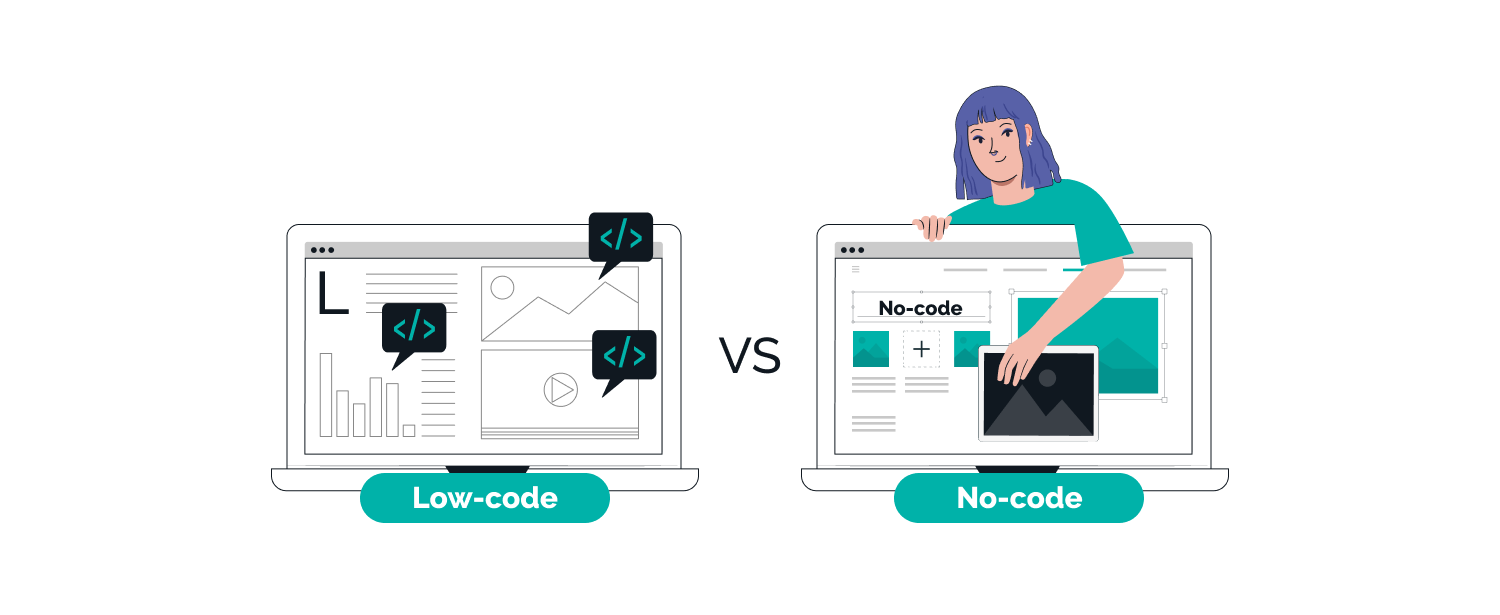
\includegraphics[width=0.75\textwidth]{cover-Low-Code.png}
\end{center}

\paragraph{}O desenvolvimento de software passou por uma revolução com a ascensão das tecnologias \textit{Low-Code} e \textit{No-Code}, duas abordagens diferentes que simplificam o processo de criação de aplicações. Enquanto ambos os métodos têm em comum o objetivo de reduzir a dependência de código manual e acelerar o desenvolvimento, suas diferenças fundamentais podem impactar significativamente a escolha entre eles e a forma de aplicá-las em diferentes contextos.\cite{bib14}

\paragraph{}O \textit{Low-Code}, como mencionado anteriormente, permite a criação de aplicações com o uso mínimo de código manual. Ele fornece uma abordagem intermediária, em que os desenvolvedores podem usar interfaces visuais e componentes pré-configurados para agilizar o processo de desenvolvimento. Esta abordagem é ideal para projetos que exigem um alto nível de personalização e flexibilidade, mas onde a velocidade de entrega e a praticidade ainda são uma prioridade. Apesar disso, \textit{Low-Code} pode apresentar algumas limitações em termos de complexidade e escalabilidade, especialmente em projetos altamente customizados ou de grande porte.\cite{bib14}

\paragraph{}Por outro lado, o \textit{No-Code} vai um passo além, eliminando completamente a necessidade de se escrever código. Isso significa que até mesmo utilizadores sem conhecimento técnico sobre programação podem criar aplicações funcionais usando de interfaces visuais intuitivas e técnicas declarativas. O \textit{No-Code} é especialmente adequado para projetos simples ou para utilizadores que procuram criar rapidamente um protótipo para uma ideia, mas pode encontrar muitas limitações em termos de personalização e complexidade.\cite{bib14}

\paragraph{}Uma diferença central entre as duas abordagens está na sua acessibilidade e facilidade de aprendizagem. Enquanto o \textit{Low-Code} requer algum nível de familiaridade com conceitos de programação e desenvolvimento de software, e pode exigir treino adicional na plataforma que está a ser usada, o \textit{No-Code} é projetado para ser tão intuitivo que até mesmo utilizadores sem experiência prévia em programação podem começar a desenvolver os seus programas imediatamente.\cite{bib14}

\paragraph{}O \textit{Low-Code} oferece mais opções de personalização e controle sobre o processo de desenvolvimento, permitindo que os desenvolvidores adaptem as soluções de acordo com as necessidades específicas de seus projetos. Por outro lado, o \textit{No-Code} pode ser mais limitado em termos de liberdade que o desenvolvedores têm, com menos opções de personalização disponíveis.\cite{bib14}



\section{Implementação de IA com Low-Code}
\subsection{\textit{Chatbot}\cite{bib8}}
\paragraph{}No desenvolvimento de aplicações/sites em \textit{Low-Code}, para ajudar o utilizador a navegar ou quando este tem alguma duvida implementa-se um \textit{Chatbot}. Um \textit{Chatbot} não passa de um programa onde está integrado uma IA\cite{bib15} capaz de simular uma conversa humana, por texto ou por voz. Alguns exemplos que vemos no dia a dia são:
\begin{itemize}
    \item \textbf{Atendimento ao cliente}\newline Quando o utilizador está com algum problema, em certos sites ou aplicações, existe um assistente virtual para o ajudar, sendo este um \textit{Chatbot}.
    \item \textbf{Bancos}\newline Alguns bancos disponibilizam de \textit{Chatbots} para algumas tarefas que não requeiram de uma pessoa.
    \item \textbf{Educação}\newline Em plantaformas de \textit{self learning} online existem \textit{Chatbots} para ajudar o utilizador a pôr em prática o que aprendeu.
    \item \textbf{Comércio online}\newline Os \textit{Chatbots} podem ser usados para localizar um produto ou ajudar o utilizador com algum problema durante as compras.
    \item \textbf{Saúde}\newline Para se fazer a marcação de uma consulta pode-se usar um \textit{Chatbot}.

\end{itemize}



\section{Soluções do Low-Code - Um pouco do que há no mercado}\label{sec7}

\paragraph{}Nos últimos anos, o mercado de plataformas de desenvolvimento \textit{low-code} tem testemunhado um crescimento significativo em resposta à demanda por soluções de desenvolvimento de software mais rápidas e eficientes. Uma variedade de empresas, desde grandes players do setor de tecnologia até startups inovadoras, têm desenvolvido e lançado suas próprias plataformas de low-code, cada uma com as suas características e funcionalidades únicas.

\paragraph{}Exploraremos algumas das principais soluções disponíveis no mercado de \textit{low-code}, oferecendo uma visão geral de suas capacidades e áreas de foco. Cada plataforma abordada aqui representa uma abordagem distinta para o desenvolvimento de software de baixo nivel, oferecendo uma gama de ferramentas e recursos para atender às necessidades de diferentes tipos de projetos e organizações.

\paragraph{}Iremos analisar com mais pormenor duas das plataformas líderes de \textit{low-code} disponíveis atualmente:
\begin{itemize}
    \item OutSystems;
    \item Zoho Creater;
\end{itemize}

\subsection{OutSystems}\label{subsec}
\begin{center}
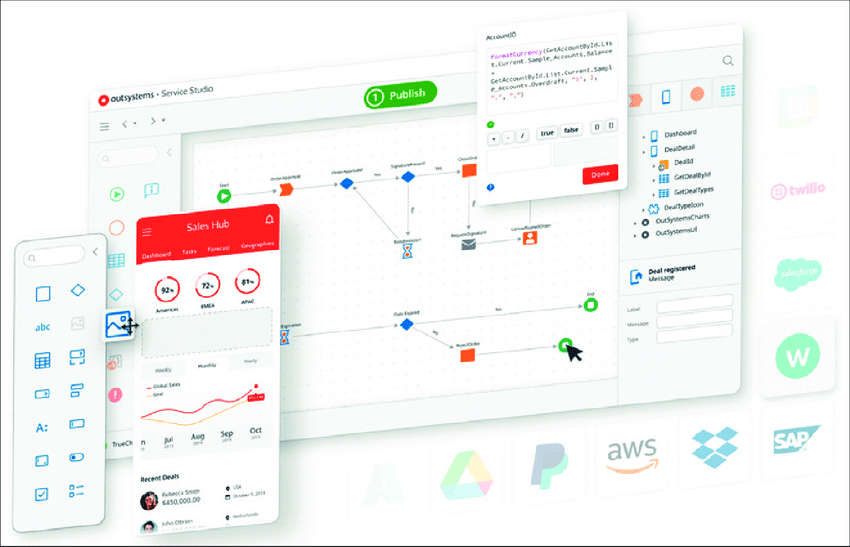
\includegraphics[width=0.75\textwidth]{LowCode-https-wwwoutsystemscom.png}
\end{center}


\paragraph{}Em 2001, OutSystems foi fundada com uma visão audaciosa: revolucionar a entrega de \textit{software}. Os seus fundadores, experientes profissionais de IT, perceberam que a maioria dos projetos de \textit{software} enfrentava problemas com prazos e orçamentos.\cite{bib9}

\paragraph{}Naquela época, predominava a abordagem "\textit{waterfall}"\cite{bib12} no desenvolvimento de software, onde mudanças tardias se tornavam cada vez mais custosas. OutSystems questionou esse paradigma, propondo uma nova abordagem: e se as mudanças fossem rápidas e económicas em qualquer estágio do ciclo de vida do \textit{software}?\cite{bib9}

\paragraph{}Essa visão levou à criação da plataforma OutSystems, projetada para tornar as alterações em aplicações rápidas, robustas e acessíveis, independentemente do tamanho do projeto. Essa abordagem ágil e flexível colocou a OutSystems na vanguarda do desenvolvimento de \textit{software}, oferecendo soluções que se adaptam dinamicamente às necessidades em constante evolução das empresas.\cite{bib9}

\paragraph{}OutSystems é uma plataforma moderna de aplicações projetadas para acelerar significativamente o desenvolvimento das aplicações mais críticas de uma empresa, oferecendo níveis sem precedentes de flexibilidade e eficiência. Desenvolvedores usam um ambiente de desenvolvimento integrado único que abrange todo o ciclo de vida do desenvolvimento: desenvolvimento, garantia de qualidade, implementação, monitorização e gerenciamento.\cite{bib11}

\paragraph{}A plataforma da OutSystems foi criada por uma equipa de profissionais de IT portugueses, com o objetivo de aproveitar todas as vantagens da abordagem \textit{low-code} no desenvolvimento de \textit{software}. Ela serve como um ambiente visual de desenvolvimento, compilador, repositório e centro de testes, proporcionando uma experiência unificada para o desenvolvimento de Web Apps, Mobile Apps e outras aplicações.\cite{bib11}

\paragraph{}A abordagem \textit{low-code} de OutSystems permite que os desenvolvedores criem aplicações de forma mais rápida e eficiente, reduzindo significativamente o tempo e os custos associados ao desenvolvimento de \textit{software} tradicional. A plataforma oferece um ambiente de desenvolvimento visual integrado, no qual os desenvolvedores podem criar a interface do utilizador, o back-end, a base de dados e a integração com sistemas ou serviços existentes de forma intuitiva e eficaz.\cite{bib11}

\paragraph{}Além disso, OutSystems fornece uma série de recursos e funcionalidades para cobrir todo o ciclo de vida do desenvolvimento de aplicações. Isso inclui suporte para desenvolvimento rápido e integração com sistemas e base de dados existentes, implementação fácil e segura de aplicações em produção, monitorização contínua da saúde das aplicações e facilidades de gerir operações diárias.\cite{bib11}

\paragraph{}A plataforma é altamente flexível e extensível, permitindo que os desenvolvedores criem uma ampla variedade de aplicações empresariais para diferentes necessidades e cenários de uso. Além disso, a OutSystems oferece suporte para a construção de aplicações móveis altamente interativos, embora possa não ser otimizada para casos de uso extremamente específicos, como jogos altamente interativos.\cite{bib10}

\subsubsection{Principais Recursos, Use Cases e Benefícios da Plataforma OutSystems}\label{subsubsec}
\paragraph{}A plataforma OutSystems oferece uma ampla gama de recursos e funcionalidades projetadas para acelerar o desenvolvimento de aplicações empresariais e impulsionar a inovação digital. Alguns dos principais recursos e benefícios que tornam a OutSystems uma solução poderosa:

\begin{itemize}
    \item \textbf{Desenvolvimento Rápido e Eficiente} \newline
    Com a abordagem \textit{low-code} de OutSystems, os desenvolvedores podem criar aplicações de forma rápida e eficiente, reduzindo significativamente o tempo necessário para o desenvolvimento. O ambiente de desenvolvimento visual integrado permite a criação de interfaces de utilizador, lógica de negócios e integrações com sistemas externos de maneira intuitiva e eficaz.\cite{bib11}
    \item \textbf{Flexibilidade e Extensibilidade} \newline
    A plataforma OutSystems é altamente flexível e extensível, permitindo que os desenvolvedores criem uma ampla variedade de aplicações empresariais para diferentes necessidades e use cases. Com suporte para uma variedade de tecnologias e integrações, as aplicações desenvolvidas em OutSystems podem ser facilmente adaptadas e expandidas para atender às necessidades em constante evolução das empresas.\cite{bib11}
    \item \textbf{Integração com Sistemas e Dados Existentes} \newline
    OutSystems oferece recursos abrangentes para integração com sistemas e dados existentes, permitindo que as aplicações desenvolvidas na plataforma se conectem facilmente a sistemas, bases de dados corporativas e serviços externos. Isso permite que as empresas aproveitem seus investimentos existentes em tecnologia e maximizem o valor de seus dados.\cite{bib11}
    \item \textbf{Implementação e Gestão Simplificados} \newline
    A plataforma OutSystems facilita a implementação e o gestão de aplicações em produção, com recursos para automação, versionamento de código e monitorização contínuo da saúde das aplicações. Isso ajuda as empresas a manter as suas aplicações funcionarem de forma eficiente e confiável, garantindo uma experiência contínua para os utilizadores finais.\cite{bib11}
\end{itemize}
\paragraph{}\textbf{Use Cases}:
\newline OutSystems é adequada para uma ampla variedade de use cases, desde aplicações empresariais internas até aplicações de consumo voltados para o cliente. Alguns exemplos incluem aplicações de CRM\cite{bib13}, gestão de inventário, automação de processos, aplicações móveis para funcionários e clientes, entre outros.\cite{bib10}

\newpage

\subsection{Zoho Creator\cite{bib16}}\label{subsec}
\begin{center}
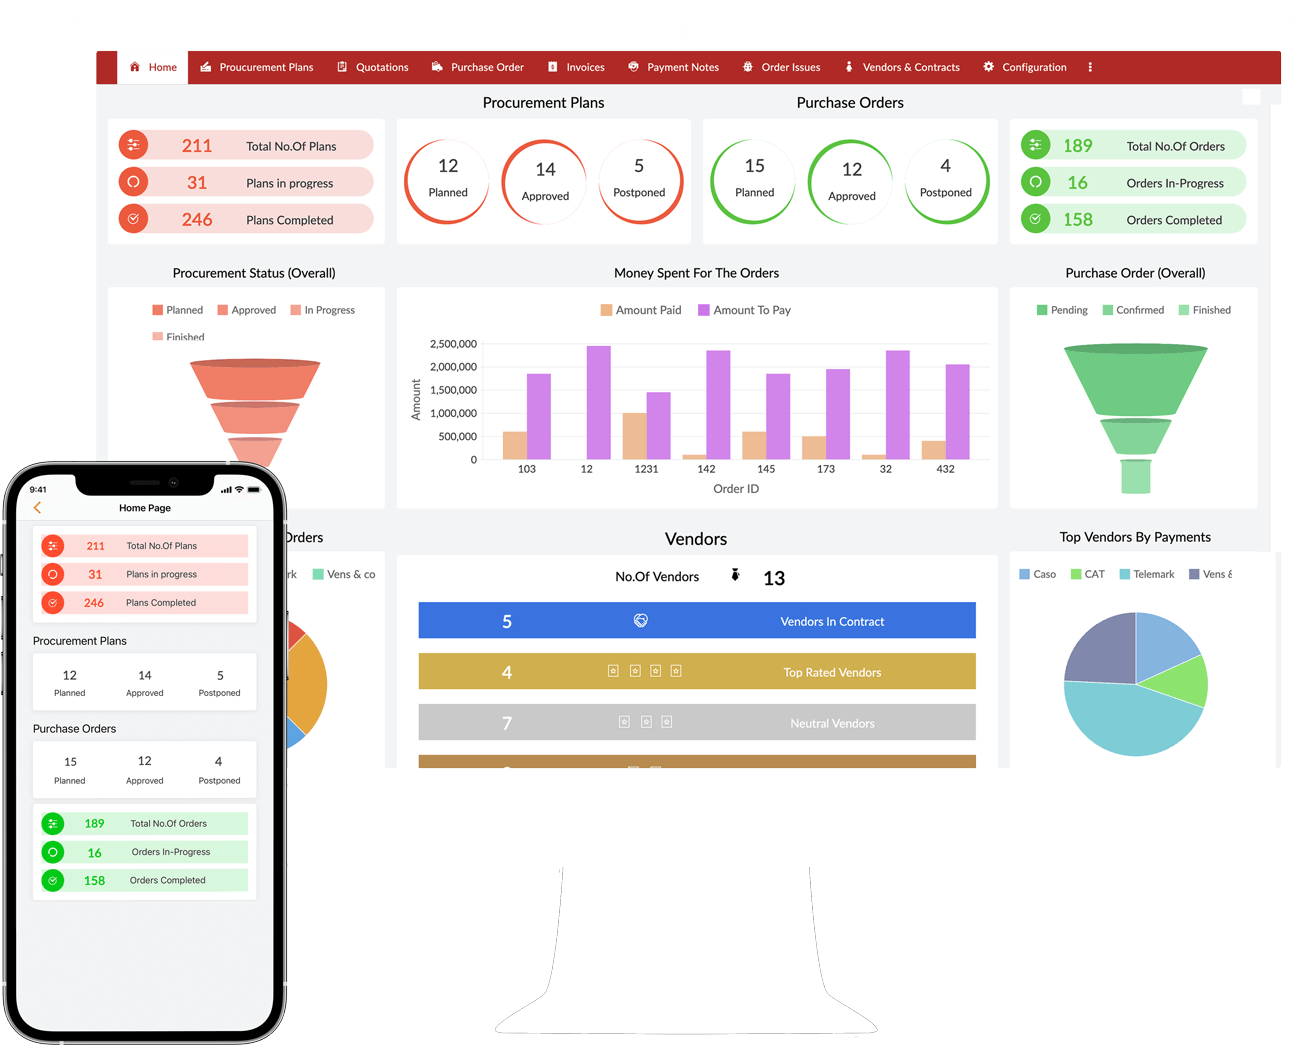
\includegraphics[width=0.75\textwidth]{build-powerfull-apps.png}
\end{center}
\paragraph{}O Zoho Creator é uma ferramenta que tal como o OutSystems serve para desenvolver aplicações em \textit{Low-Code}. A Zoho, antigamente chamada de AdventNet, Inc., foi fundada em 1996. O Zoho Creator foi criado em 2006 usado só pela sua empresa.
\paragraph{}Uma das vantagens do Zoho Creator é a sua acessibilidade, uma vez que pode ser acedido pele \textit{web} ou por aplocações para Android ou iOS.
\paragraph{}Em comparação com Outsystems o Zoho Creator tem uma configuração mais fácil, não precisa de qualquer tipo de treino ou curso para se começar a usar, o construtor é totalmente basiado na \textit{cloud} e \textit{updates} e \textit{backups} automáticos.
\paragraph{}\textbf{O Zoho Creator premite:}
\begin{itemize}
    \item Criação de aplicações consuante a necessidade do utilizador
    \item Automação de fluxo de trabalho com facilidade
    \item Conectar ou extender outras aplicações
\end{itemize}

\newpage

\paragraph{}\textbf{Use Cases}:
\newline O Zoho Creator é ideal para um uso abrangente, desde aplicações empresariais até aplicações de consumo voltados para o cliente. Alguns exemplos incluem aplicações de CRM\cite{bib13}, usar IA, como \textit{Chatbots}, nas suas aplicações, automação de processos, aplicações móveis, obter relatórtio e \textit{insights} a tempo real, entre outros.



\section{Conclusão}\label{sec8}

\paragraph{}O \textit{Low-Code} representa uma mudança significativa na forma como o \textit{software} é desenvolvido e implementado, oferecendo uma abordagem mais rápida, eficiente e acessível para a criação de aplicações. Ao simplificar o processo de desenvolvimento, o \textit{Low-Code} permite que as empresas acelerem a entrega de soluções de \textit{software}, aumentem a produtividade das equipas de desenvolvimento e ofereçam uma experiência de mercado mais ágil e eficiente para os consumidores finais.

\paragraph{}No entanto, é importante reconhecer que o \textit{Low-Code} não é uma solução única para todos os problemas de desenvolvimento de \textit{software}. Existem casos em que a programação manual pode ser necessária para lidar com requisitos complexos ou personalizados. Portanto, é essencial avaliar cuidadosamente as necessidades de cada projeto e escolher a abordagem de desenvolvimento mais adequada.

\paragraph{}Além disso, o \textit{Low-Code} tem potencial para promover a inclusão digital, permitindo que pessoas com pouca ou nenhuma experiência em programação contribuam para o desenvolvimento de aplicações. Isso pode levar a uma democratização do desenvolvimento de software, abrindo portas para uma gama mais ampla de talentos e perspectivas.

\paragraph{}Para futuras investigações, áreas interessantes a serem exploradas incluem a integração de \textit{Low-Code} com inteligência artificial para automação de processos, o impacto do \textit{Low-Code} na agilidade e inovação das empresas e o desenvolvimento de aplicações específicas para setores como saúde, educação e finanças.

\paragraph{}Em suma, o \textit{Low-Code} está posicionado para continuar a moldar o futuro do desenvolvimento de \textit{software} nos próximos anos, oferecendo oportunidades emocionantes para inovação, crescimento e inclusão.


\newpage
\bibliographystyle{plain}
\bibliography{sn-bibliography}

\end{document}